\chapter{Bestimmung der Lasten nach CS 23}\label{cha:Bestimmung der Lasten nach CS 23}

\section{Ausgangsannahmen für das Fluggerät}

\subsection{Sicherheiten und Anforderungen}

Für die Berechnung der Lasten und Dimensionierungen wird von den Sicherheiten und Anforderungen an das Flugzeug aus Tabelle \ref{} im Anhang ausgegangen.

\subsection{Der Tragflügel}

Der Tragflügel wird für eine Flugaufgabe mit folgenden Parametern ausgelegt:

\begin{table}[h]
\centering
\begin{tabular}{|l|l|l|l|}
\hline
Parameter  & Bezeichnung &  Wert & Einheit \\ \hline
Fluggeschwindigkeit  & $V_{reise}$ & 15,0 & $m/s$\\ \hline
Abbfluggewicht & $m_{reise}$  & 5,0 & $kg$\\ \hline
Profilierung & Clark-Y & - & - \\ \hline
Segmentteilung & $Y_{seg}$ & 700 & mm\\ \hline
\end{tabular}
\caption{Grundannahmen für den Tragflügel}
\label{tab:Grundannahmen für den Tragflügel}
\end{table}
Die Fläche setzt sich aus einem Zentralen Rechtecksegment und jeweils angeschlossenem Außenflügel 
in Trapezform zusammen.
Hierbei werden Eigenschaften von bisher Eingesetzten Flügel übernommen.
Eine Disskussion über die Wahl dieser Aerodynamischen Parameter findet in dieser Arbeit nicht statt. 
Es wird von der Strukturauslegung ausgegangen.
Die Wahl der geradlinig aufgebauten Tragflächensegmente ermöglicht hier Vorteile bei der Fertigung.

Im Bild \ref{} ist ein Aufriss mit den Grundabmessungen dargestellt.

\begin{table}[h]
\centering
\begin{tabular}{|l|l|l|l|}
\hline
Parameter  & Bezeichnung &  Wert & Einheit \\ \hline
Spannweite  & $V_{reise}$ & 2800 & $mm$\\ \hline
Projizierte Fläche & $A_{ref}$  & 0,752 & $m^2$\\ \hline
Wurzeltiefe & $CH_{Wurzel}$ & 300 & $mm$ \\ \hline
Spitzenverwindung & $\alpha_{Spitze}$ & -\,2 & $^\circ$\\ \hline
Mittlere Flügeltiefe & $l_{\mu}$ & 275 & $mm$ \\ \hline
\end{tabular}
\caption{Dimensionen des Tragflügels}
\label{tab:Dimensionen des Tragflügels}
\end{table}

\section{Bestimmung der Lasten}

Mit seinem Gewicht von 5,0 Kg fällt der Flieger nach CS 23 in die Kategorie "Normal".
Alle Auslegungsrechnungen basieren auf dieser Einordnung.

\subsection{Lasten im stationären Flug}

Im folgenden zeigt die Abbildung \ref{fig:Stationärer Reiseflug in XFLR} den Aeroynamischen Entwurf im Stationär ausgelegten Reiseflug.

\begin{figure}[H]
\centering
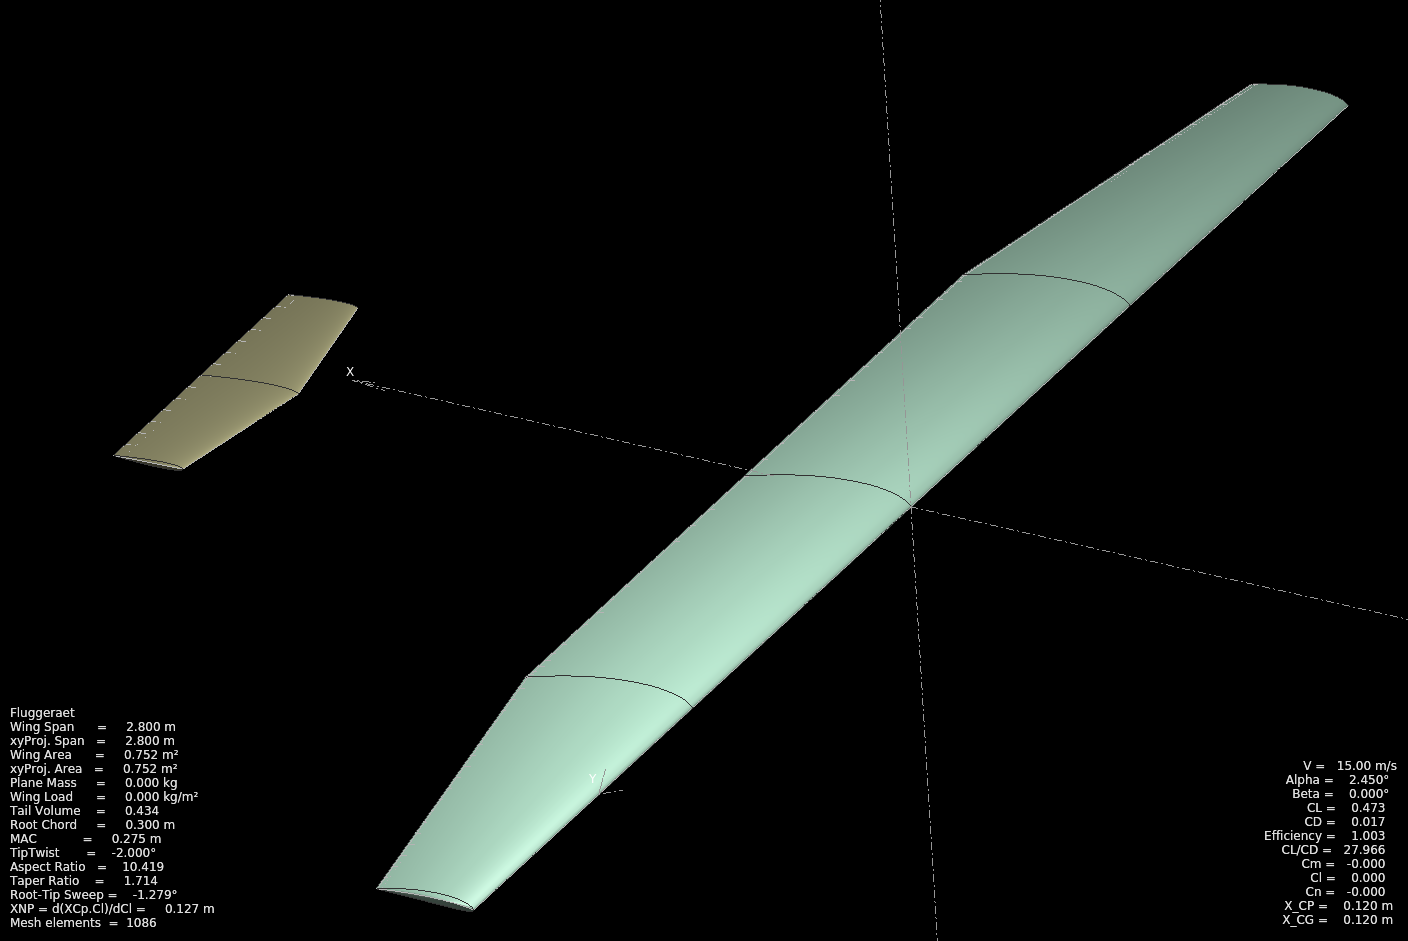
\includegraphics[width=0.9\textwidth]{bilder/Fotos/Aeroentwurf_Fluegelkonstruktion.png}
\caption{Stationärer Reiseflug bei 15 $m/s$ in der XFLR Berechnung} 
\label{fig:Stationärer Reiseflug in XFLR}
\end{figure}

In diesem Fall ergibt die Ermittlung der Aerodynamischen Beiwerte folgende Situation:

\begin{table}[h]
\centering
\begin{tabular}{|l|l|l|l|}
\hline
Parameter  & Bezeichnung &  Wert & Einheit \\ \hline
Fluggeschwindigkeit  & $V_{reise}$ & 15,00 & $m/s$\\ \hline
Abbfluggewicht & $m_{reise}$  & 5,0 & $kg$\\ \hline
Anstellwinkel & $\alpha$ & 2,45 & $^\circ$ \\ \hline
Auftriebsbeiwert & $C_{L}$ & 0,473 & -\\ \hline
Widerstandsbeiwert & $C_{D}$ & 0,016  & -  \\ \hline
\end{tabular}
\caption{Errechnete Werte im Stationären Reiseflug}
\label{tab:Errechnete Werte im Stationären Reiseflug}
\end{table}

In diesem Zustand ist der Flügel frei von Nickmomenten und das Höhenleitwerk erzeugt keine Aerodynamischen Auftriebskräfte.



\subsection{Kritische Lasten}

Nach CS 23.337 werden das positive und negative maximale Manöver Lastvielfache berechnet.
\begin{figure}[H]
\centering
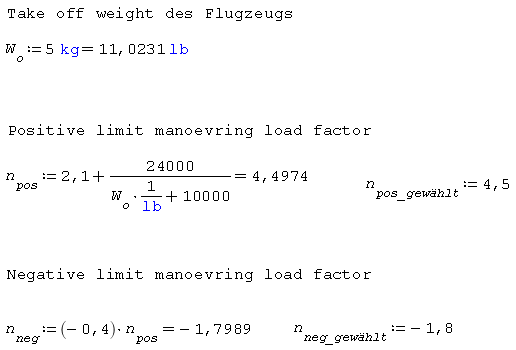
\includegraphics[width=0.9\textwidth]{bilder/Formeln/Kritische_Lastfaelle_Manoeverlasten.png}
\caption{Limit manoevring load factors nach CS23.337} 
\label{fig:Limit manoevring load factors nach CS23.337}
\end{figure}

%/Hochstart

%/Hier soll in konservativer Auslegung der Lasten für den gegebenfalls belastendensten Fall beim Hochstart mittels Gummiseil abgeschätzt werden. Hier übersteigt die Auftriebsbelastung für den Hochanstellwinkelbereich kurzeitig den Maximalauftrieb des Profils durch den Betrieb im instationären Bereich./%


\subsection{Betriebsgrenzen des Tragflügels}

Der Einsatz des Tragwerks unterliegt sowohl aerodynamischen als auch mechanischen Grenzen im Betrieb.

Zunächst werden die kritischen Geschwindikeiten für den Einsatz mit und Ohne Klappeneinsatz bestimmt.

\begin{figure}[H]
\centering
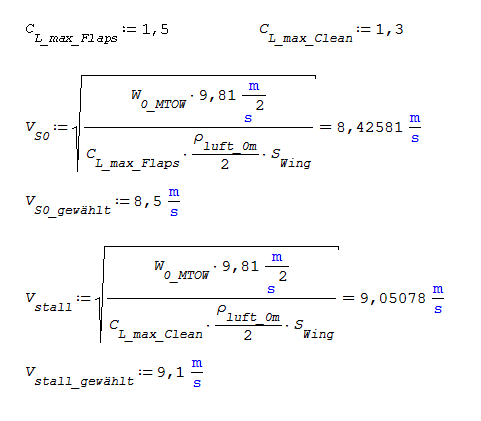
\includegraphics[width=0.9\textwidth]{bilder/Formeln/Mindestbetriebsgeschwindikeit.png}
\caption{Kritische Fluggeschwindikeiten} 
\label{fig:Kritische Fluggeschwindikeiten}
\end{figure}

Im selben Verfahren wird die Stallgeschwindikeit für negative Auftriebe Bestimmt.

\begin{figure}[H]
\centering
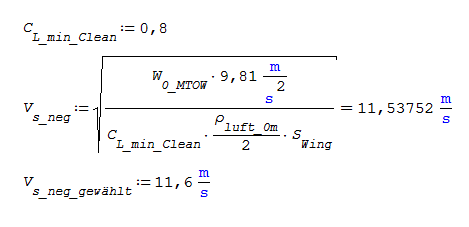
\includegraphics[width=0.9\textwidth]{bilder/Formeln/VS_neg.png}
\caption{Mindestgeschwindikeit für Invertierten Flug} 
\label{fig:Mindestgeschwindikeit für Invertierten Flug}
\end{figure}

Aus den Parametern ergibt sich im weiteren die mindestens geforderte Höchstgeschwindigkeit für den Klappeneinsatz.

\begin{figure}[H]
\centering
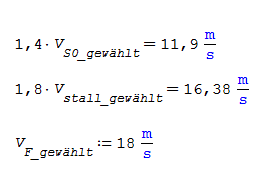
\includegraphics[width=0.9\textwidth]{bilder/Formeln/VF.png}
\caption{Klappenhöchstgeschwindigkeit} 
\label{fig:Klappenhöchstgeschwindigkeit}
\end{figure}

Des weiteren ergeben sich die Manövergeschwindigkeiten $V_{A}$ und $V_{G}$ nach (CS 23.335).


\begin{figure}[H]
\centering
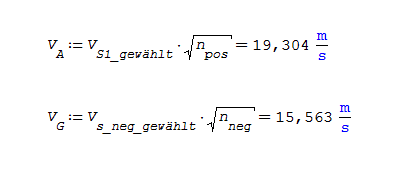
\includegraphics[width=0.9\textwidth]{bilder/Formeln/V_g.png}
\caption{Manövergeschwindigkeiten} 
\label{fig:Manövergeschwindigkeiten}
\end{figure}
